\chapter{Map Data Sources}\label{chap:mapdatasources}

\textcolor{orange}{Notater:}
hva dette kapittelet er... hvorfor vi trenger data... hvordan vi fikk datakildene... 
Data var VELDIG sentralt i prosjektet, 
\begin{itemize}
    \item Ikke våre data, men de er tilgjengelige åpent, noen under NLOD.
    \item Sammenkoble forskjellige datakilder
\end{itemize}

Building on the architectural overview and core functionality described previously, the following chapter introduces the spatial and environmental data sources that form the foundation of the application and its trafficability assessments. Since the system relies entirely on external datasets, data quality and availability were critical to the project's success. We used publicly accessible data from Norwegian agencies, all of which are licensed under NLOD\footnote{\url{https://data.norge.no/nlod}}, ensuring open use. The chapter describes each dataset and explains how they were combined to create an integrated mapping solution. Multiple layers, including both raster and vector formats, were used to visualize geological and meteorological factors. These include superficial deposits, frost depth, and water saturation levels, all of which affect forestry road conditions. The data is presented through a composite map interface that lets users view and interact with different layers. The backend service alters this data further by fusing it into a final trafficability classification. Together, these map layers form the foundation for forecasting road usability and planning forestry operations.

\section{Map Layers}\label{sec:maplayers}

% KANKJE GLOSSARY FOR "COMPOSITE MAP"
The interactive map on the website supports multiple layers, allowing the user to build a composite map with various types of data. These layers include both meteorological and geological data relevant to assessing road conditions and the surrounding environment.

\subsection{Base Layers}\label{subsec:baselayers}

The user has the option to change the base layer of the map. In the current version, two options are available: the standard map from \gls{openstreetmap}\footnote{\url{https://www.openstreetmap.org}} and the terrain map from OpenTopoMap\footnote{\url{https://opentopomap.org}}. This flexibility allows users to choose the base layer that best suits their task. For example, the standard map shown in \autoref{fig:maplayer:standardlayer} provides a clean, general-purpose view that is ideal for navigation and overlaying vector data. In contrast, the terrain map shown in \autoref{fig:maplayers:topolayer} includes elevation and contour information, making it more suitable for geographic or environmental analysis. Offering multiple base layers enhances usability across a wider range of scenarios and user preferences.

\begin{figure}[h]
     \centering
     \begin{subfigure}[b]{0.45\textwidth}
         \centering
         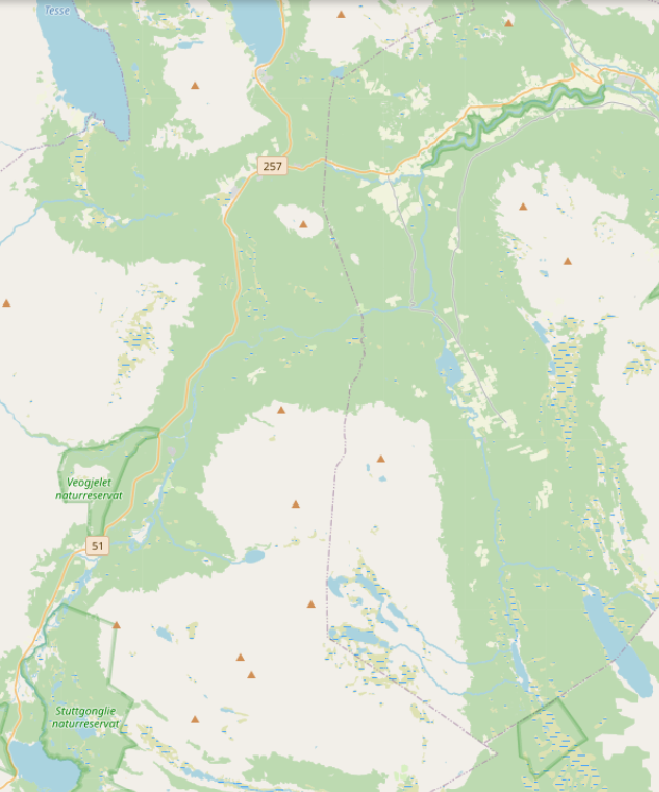
\includegraphics[width=\textwidth]{figures/base_layer_standard.pdf}
         \caption{Standard base layer}
         \label{fig:maplayer:standardlayer}
     \end{subfigure}
     \hfill
     \begin{subfigure}[b]{0.45\textwidth}
         \centering
         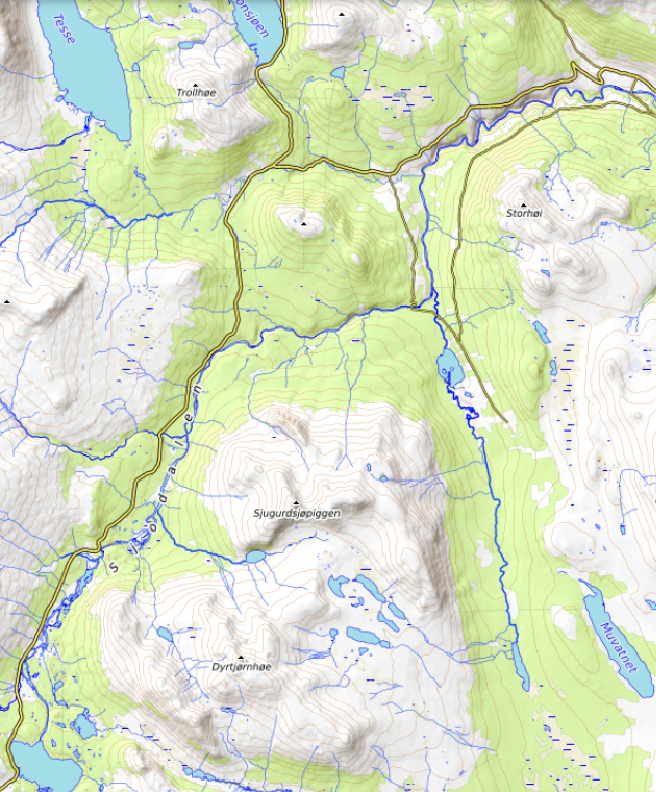
\includegraphics[width=\textwidth]{figures/base_layer_topo.pdf}
         \caption{Terrain base layer}
         \label{fig:maplayers:topolayer}
     \end{subfigure}
    \caption{Base map layer options}
    \label{fig:maplayer:baselayers}
\end{figure}

\subsection{Superficial Deposits}\label{subsec:superficialdeposits}

The map layer, showing superficial deposits, is provided by \acrfull{ngu}\footnote{\url{https://www.ngu.no/en}}. The superficial deposits data provide information on the distribution of surface sediments covering bedrock, mainly formed during and after the last Ice Age. It represents the dominant soil type in the upper layers, but does not account for deeper variations. The mapped soil types include stones, gravel, sand, clay, peat, and \gls{moraine} material \cite{geonorge_losmasser}. Because different soil types vary in their load-bearing capacity, this layer is valuable for assessing the trafficability of forestry roads.

The various soil types are visualized using different colors, as shown in \autoref{fig:maplayer:superficialdeposit}. Each main soil category is assigned a base color, while subtypes are distinguished by varying shades. For example, moraine is represented in green, with thick moraine shown as a darker shade and thin moraine as a lighter one. Given the large number of subtypes, a complete overview of the colors and corresponding soil types is included in \autoref{appendix:superficial_deposits_colors}, which is provided by NGU \cite{ngu_løsmasser_tegneregler}.

\begin{figure}[h]
    \centering
    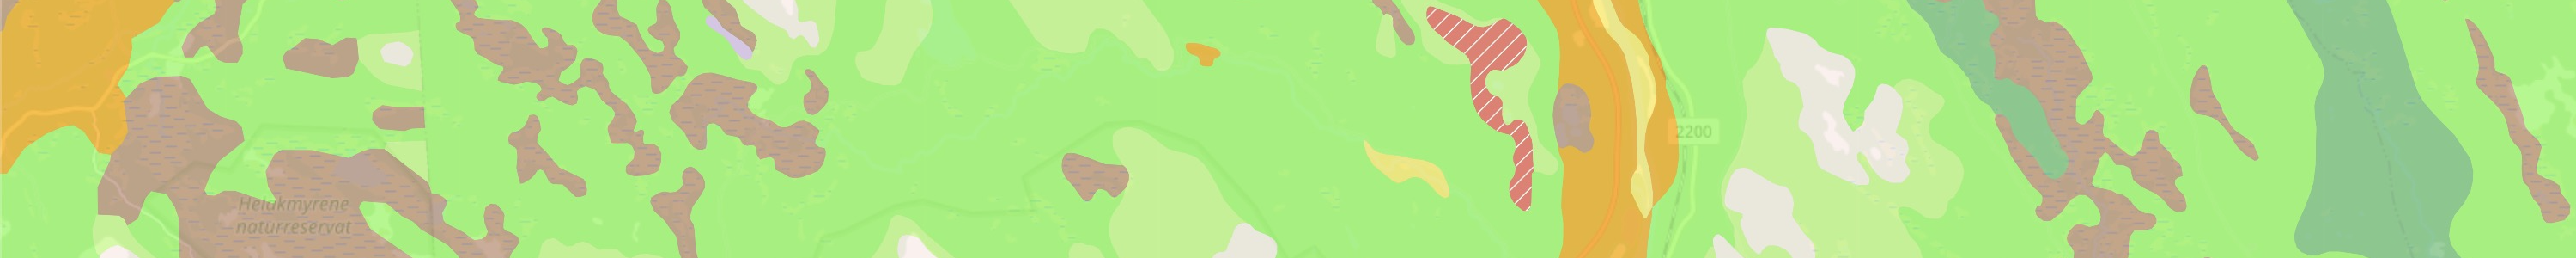
\includegraphics[width=1\linewidth]{images/maplayers/superficialdeposits.png}
    \caption{Example of the superficial deposits map layer}
    \label{fig:maplayer:superficialdeposit}
\end{figure}

\subsection{Frost Depth}\label{subsec:frostdepth}

The frost depth map layer, provided by \acrfull{nve}\footnote{\url{https://www.nve.no/english}}, visualizes frost depth as a raster map, with colors ranging from dark blue (indicating deep frost) to light green (indicating no frost). This layer is particularly useful for assessing the trafficability of forestry roads. When frost depth reaches \qty{10}{\centi\meter} or more (see \autoref{tab:frost_depth_classification}), it overrides other factors, and road conditions are generally suitable for heavy vehicles. However, in the absence of sufficient frost, other map layers become critical for evaluating trafficability. Consequently, most forestry roads tend to have good trafficability throughout the Norwegian winter, when frost is typically present \cite{wiki:tele}.

% KANSKJE GI EKSEMPLER PÅ NÅR (OG HVOR) DET ER VANLIG MED DE FORSKJELLIGE DYBDENE
\begin{table}[h]
    \centering
    \begin{tabular}{|l|l|l|}
        \hline  
        \textbf{Color} & \textbf{Frost Depth} & \textbf{Depth} \\
        \hline
        \cellcolor[HTML]{00009c} & Very Deep Frost & > 75 cm \\
        \hline
        \cellcolor[HTML]{0018ff} & Deep Frost & 30-75 cm \\
        \hline
        \cellcolor[HTML]{009aff} & Frost & 10-30 cm \\
        \hline
        \cellcolor[HTML]{84ebff} & Shallow Frost & 5-10 cm \\
        \hline
        \cellcolor[HTML]{deffff} & Partially Frost-free & 0-5 cm \\
        \hline
        \cellcolor[HTML]{cef77b} & No Frost & 0 cm \\
        \hline
    \end{tabular}
    \caption[Frost depth classification and corresponding colors]{Frost depth classification and corresponding colors, as defined by \acrshort{nve} \cite{nve2025waterdata}}
    \label{tab:frost_depth_classification}
\end{table}

An example of the frost depth map layer as it appears on the website is shown in \autoref{fig:maplayer:frostdepth}. The dataset includes both historic and forecasted data, spanning from 1957 to nine days into the future, and represents daily averages. The data is presented as a raster grid with a spatial resolution of $1 \times 1$ km. The color-coded visualization enables users to quickly assess ground conditions based on frost depth, as defined in \autoref{tab:frost_depth_classification}. This makes it particularly useful for identifying seasonal and regional variations in frost conditions.

\begin{figure}[h]
    \centering
    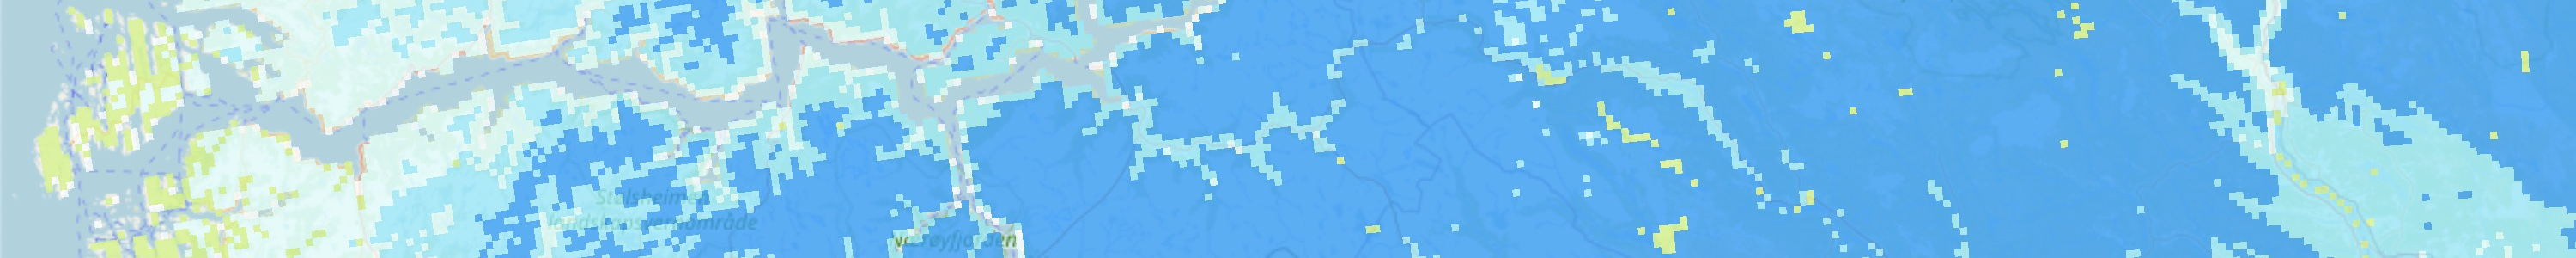
\includegraphics[width=1\linewidth]{images/maplayers/frostdepth.png}
    \caption{Example of the frost depth map layer}
    \label{fig:maplayer:frostdepth}
\end{figure}

\subsection{Soil Saturation}\label{subsec:soilsaturation}

The soil saturation data, provided by \acrshort{nve}, represents the ratio between the current simulated water content in the \gls{groundwater} and \gls{rootzone} and the highest values observed during the historical reference period from 1981 to 2010 \cite{nve2025waterdata}. The \gls{groundwater} zone refers to the soil level that is fully saturated, while the \gls{rootzone} lies above it and is typically not fully saturated. For example, a soil saturation level of \qty{70}{\percent} indicates that the soil currently holds \qty{70}{\percent} of the maximum water content recorded during the reference period. An example of how to soil saturation map layer looks like is shown in \autoref{fig:maplayer:soilsaturation}.

\begin{figure}[h]
    \centering
    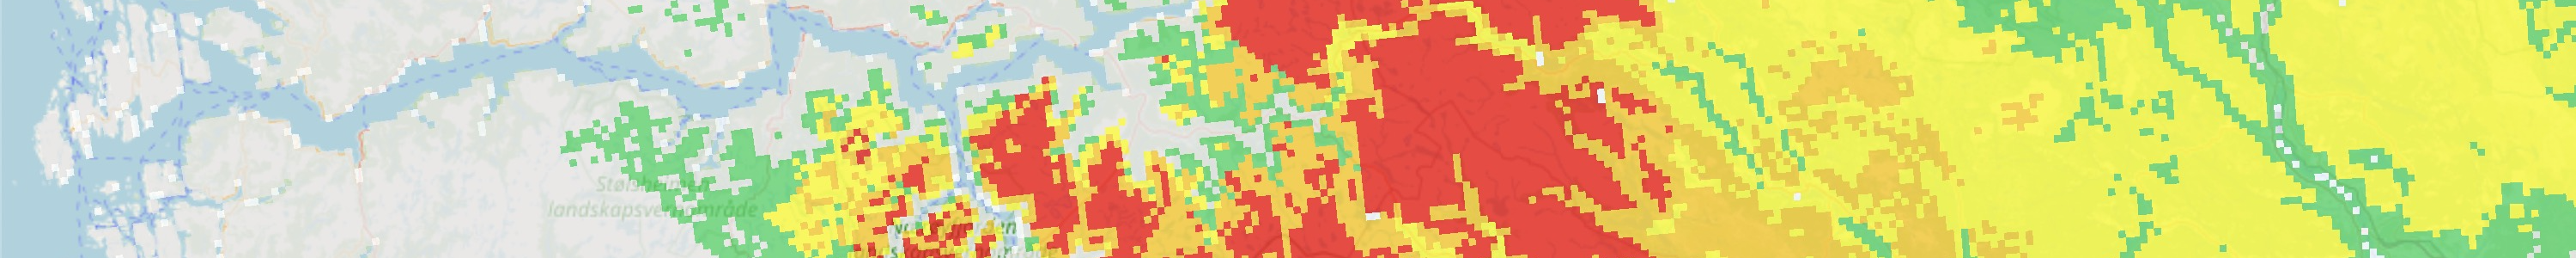
\includegraphics[width=1\linewidth]{images/maplayers/soilmoisture.png}
    \caption{Example of the soil saturation layer}
    \label{fig:maplayer:soilsaturation}
\end{figure}

Soil saturation can be used to assess \gls{trafficability}, which in this context refers to the highest level of soil moisture a road can tolerate without experiencing excessive deformation and potentially lead to dangerous driving conditions. This threshold varies depending on the type of superficial deposits present, as different materials have varying levels of permeability \cite{fjeld2023trafficability}. \textcolor{orange}{legge til at vi kun fokuserer på stedegne masser?}. The dataset covers the same temporal range as the frost depth data, from 1957 to nine days into the future, and also provides daily averages based on a 24-hour period. Like the frost depth dataset, it is presented as a raster grid with a spatial resolution of $1 \times 1$ km. \acrshort{nve} categorizes soil moisture into distinct levels, as shown in \autoref{tab:soil_saturation_classification}, with the most extreme levels (i.e., the upper percentage range) typically occurring after prolonged rainfall or frost thaw in the spring.

\begin{table}[h]
    \centering
    \begin{tabular}{|l|l|}
        \hline  
        \textbf{Color} & \textbf{Soil Saturation} \\
        \hline
        \cellcolor[HTML]{f82200} & Above 90\% \\
        \hline
        \cellcolor[HTML]{f8c400} & 80 - 90\% \\
        \hline
        \cellcolor[HTML]{f8fc00} & 70 - 80\% \\
        \hline
        \cellcolor[HTML]{29d460} & 60 - 70\% \\
        \hline
        \cellcolor[HTML]{e4e4e4} & Under 60\% \\
        \hline
    \end{tabular}
    \caption[Soil saturation classification and corresponding colors]{Soil saturation classification and corresponding colors, as defined by \acrshort{nve} \cite{nve2025waterdata}}
    \label{tab:soil_saturation_classification}
\end{table}

\subsection{Forestry Roads}

\textcolor{orange}{nevn at det er (relativt) statisk} 

The forestry roads map layer is the only layer modified by the backend server. This layer is based on a vector dataset retrieved via a \gls{wfs} service in \gls{geojson} format, provided by GeoNorge\footnote{\url{https://www.geonorge.no/en}} and Kartverket\footnote{\url{https://www.kartverket.no/en}}. In the \gls{geojson}, forestry roads are represented as geometric LineString features, where each LineString defines a segment between two coordinates. Often, a single road is divided into multiple such segments. Each feature also includes properties such as road number, municipality number, and feature length.

The backend server alters this \gls{geojson} by adding additional properties derived from other map layers described earlier (\ref{subsec:superficialdeposits}, \ref{subsec:frostdepth}, and \ref{subsec:soilsaturation}). Another data source incorporated into the forestry roads layer is Fjordkatalogen\footnote{\url{https://kartkatalog.miljodirektoratet.no/MapService/Details/fjordkatalogen}} from the Norwegian Environment Agency\footnote{\url{https://www.environmentagency.no/}}, which will be detailed later in \autoref{sec:implementation:server}. 

By combining information from these layers, the backend classifies the load-bearing capacity, or \gls{trafficability}, of the roads. Trafficability is visually indicated by road colors: green for safe, yellow for cautious, and red for unsafe, as shown in \autoref{fig:maplayer:forestryroads}. The detailed implementation of the Forestry Roads service is explained later in \autoref{chap:implementation}.

\begin{figure}[h]
\centering
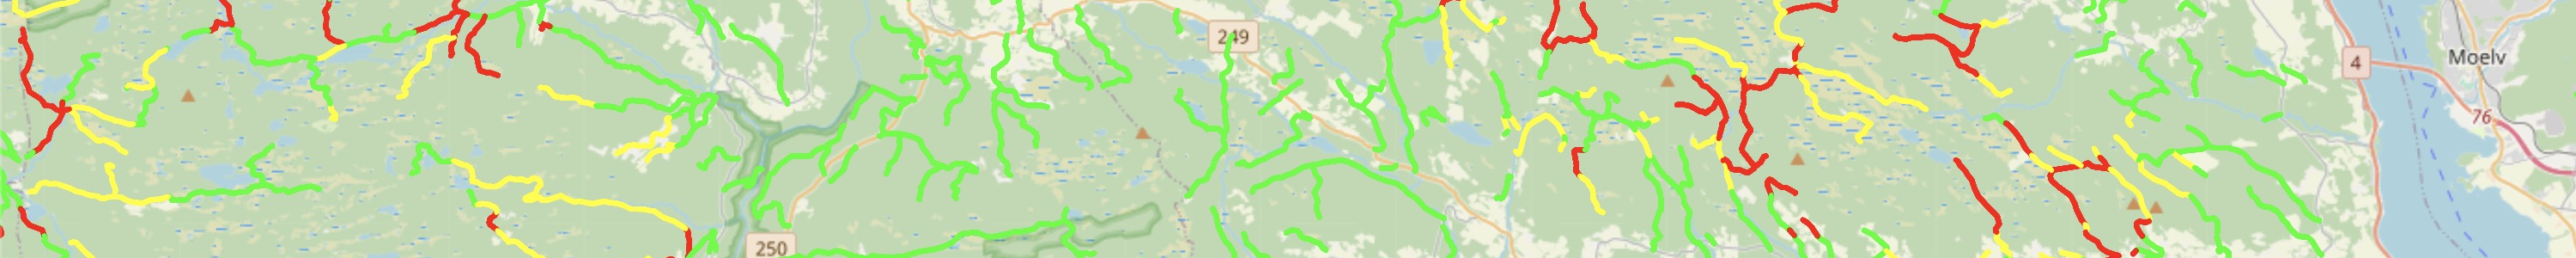
\includegraphics[width=1\linewidth]{images/maplayers/forestryroad.png}
\caption{Example of the forestry roads map layer}
\label{fig:maplayer:forestryroads}
\end{figure}

\subsection{Soil Moisture}

Soil moisture provided by, \acrfull{nibio}\footnote{\url{https://www.nibio.no/}}, is represented as a static raster map indicating areas with the highest likelihood of increased moisture content in the ground. The map highlights zones with a higher risk of deformation of roads and potential impacts on water quality during forestry operations. It is divided into several soil moisture classes, based on the elevation difference in centimeters between a given point and the nearest point estimated to be saturated with water. Soil moisture levels are visualized using a graded color scale shown in \autoref{tab:soil_moisture_classification}. The map accounts for surface terrain slope but does not consider superficial deposits \cite{geonorge_soil_moisture}.

\begin{table}[h]
    \centering
    \begin{tabular}{|l|l|}
        \hline  
        \textbf{Color} & \textbf{Soil Moisture} \\
        \hline
        \cellcolor[HTML]{000080} & Water \\
        \hline
        \cellcolor[HTML]{0000ff} & 0 - 25 cm \\
        \hline
        \cellcolor[HTML]{1e90ff} & 25 - 50 cm \\
        \hline
        \cellcolor[HTML]{00bfff} & 50 - 75 cm \\
        \hline
        \cellcolor[HTML]{87cefa} & 75 - 100 cm \\
        \hline
        \cellcolor[HTML]{ffffff} & > 100 cm \\
        \hline
    \end{tabular}
    \caption[Soil moisture classification and corresponding colors]{Soil moisture classification and corresponding colors, as defined by \acrshort{nibio} \cite{geonorge_soil_moisture}}
    \label{tab:soil_moisture_classification}
\end{table}

The soil moisture layer has a resolution of $1 \times 1$m which makes it especially useful for identifying terrain that is more prone to becoming saturated under wet conditions. When combined with dynamic soil saturation data, it becomes an even more valuable tool, particularly during periods of heavy precipitation or frost thaw. Transport manager can use this map layer to manually inspect the conditions of a potential forestry operation area, by manually checking where increased moisture content could impact the trafficability. An example of the soil moisture layer as visualized in the application is shown in \autoref{fig:soil_moisture_example} where the darker shades of blue indicate a higher likelihood of increased moisture content.

\begin{figure}[h]
    \centering
    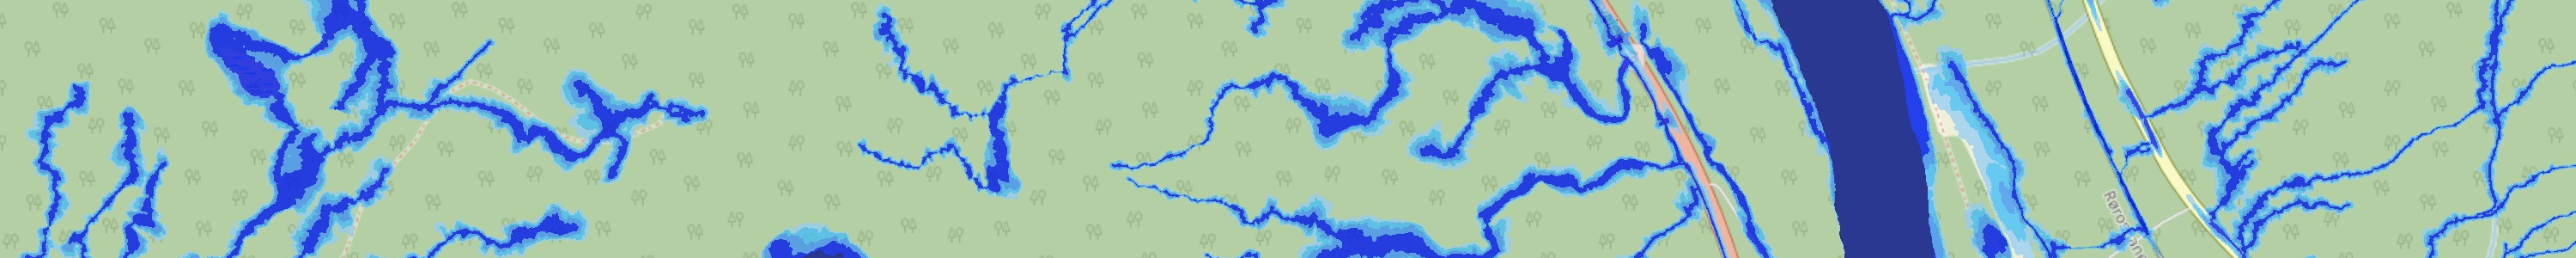
\includegraphics[width=1\linewidth]{images/maplayers/markfuktighet.png}
    \caption{Example of the soil moisture layer}
    \label{fig:soil_moisture_example}
\end{figure}

\section{Gridded Water Balance Model}

The Gridded Water Balance (GWB) model is used to compute hydrological variables displayed on the SeNorge\footnote{\url{https://www.senorge.no}} grid maps. It is a spatially distributed version of the HBV model, originally developed for flood prediction, and calculates the water balance individually for each \qty{1}{\kilo\meter\squared} grid cell \cite{nve2025waterdata}.

Each cell in the grid is defined by its mean elevation and the proportions of various land cover types, such as vegetation, soil, wetlands, lakes, and glaciers. The model runs on a daily basis, using gridded temperature and precipitation data as input \cite{nve2025waterdata}.

The GWB model simulates processes including snow accumulation, moisture in the root zone, groundwater storage, evaporation, surface runoff into rivers, wetlands, and lakes, as well as frost depth and glacier dynamics. Potential evaporation is estimated using air temperature and vegetation growth during the growing season, while actual evaporation depends on the availability of soil moisture \cite{nve2025waterdata}.

Each grid cell's water balance is calculated independently. Parameters are adapted per cell to account for differences in terrain, vegetation, and soil composition, ensuring that local hydrological behavior is realistically represented \cite{nve2025waterdata}.

The GWB model is also the basis for the frost depth and soil moisture saturation map layers provided by SeNorge and NVE.

\section{Sources of Uncertainty}\label{sec:mapdatasources:sourcesofuncertainty}

\textcolor{orange}{Gjerne skriv om feilkilder fra andre en senorge dataen: SHAPE data (løsmasse, fjord), unøyaktige veidata, }

Various factors contribute to uncertainties in the frost depth and soil saturation maps. These include possible errors in the interpolation of meteorological and soil data, as well as limitations in how the model translates real-world conditions. These uncertainties are especially important around the freezing point (\qty{0}{\celsius}), where even minor temperature variations can influence whether precipitation falls as rain or snow, or if snow begins to melt \cite{senorge_watermap}. The frost depth map tends to provide more accurate simulations of soil freezing compared to soil thawing \cite{nve2025waterdata}.

Localized weather events, such as isolated rain showers missed by nearby weather stations, may also go unnoticed. Furthermore, environmental factors like wind, humidity, and solar radiation, which are not accounted for in the model, can speed up snowmelt, causing discrepancies between the model's predictions and actual conditions \cite{senorge_watermap}.

The SeNorge maps (frost depth and water saturation) show daily averages, which may miss short-term variations like intense rainfall or rapid changes in temperature within a single day. The forecast maps predict up to nine days ahead, with increasing uncertainty the further into the future the prediction extends. Finally, the model's representation of vegetation and soil types may not always be accurate, potentially leading to the overestimation or underestimation of soil saturation levels \cite{senorge_watermap}.

\section{Unused Data Sources}\label{sec:unuseddatasources}

During the preliminary research phase, multiple potential data sources were found in addition to what the ones the \gls{productowner} had knowledge of. The sources detailed in this section were the most promising ones, and were either considered or tested in the application. Although they were ultimately left unused, these sources may still hold value for future iterations of the project.

\subsection{Open-Meteo}

One such potential data source was Open-Meteo\footnote{\url{https://open-meteo.com/}}. Open-Meteo is an open-source weather API that offers free access for non-commercial use \cite{openmeteo}. Open-Meteo offers an expansive range of meteorological data, including historical and forecasts of soil moisture and soil temperature. These variables are central to modeling trafficability \cite{fjeld2023trafficability}, but the spatial resolution of \qty{25}{\kilo\meter\squared} would not give an accurate representation of the conditions in each road. Additional sanity checks of critical periods like thawing and heavy rains suggested that the data could be unreliable. Although Open-Meteo offers great usability and large amounts of data, the spatial resolution and quality of our required data did not meet the application's requirements, and was ultimately left unused. 

\subsection{Satellite Data}

Another source of data that was investigated was data from satellites. Satellite data was originally meant to be the main source of data, as there were some key advantages. According to a nationwide pilot study by \textcite{fjeld2023trafficability}, superficial deposit characteristics,
\acrshort{nasa} \gls{smap}\footnote{\url{https://www.earthdata.nasa.gov/data/instruments/smap-l-band-radiometer}}, \acrfull{swi} from \gls{sentinel-1}\footnote{\url{https://land.copernicus.eu/en/products/soil-moisture}}, in addition to \gls{groundwater} level can explain up to \qty{70}{\percent} of the variation of forest road trafficability \cite{fjeld2023trafficability}. Satellite data is also a measured value, instead of a modeled, potentially increasing the accuracy of the data.

After exploring the use of satellite data, it became clear that it wasn't a good fit for this project. The spatial resolution of satellite data is too large to be applied at a local scale, ranging from \qty{25}{} to \qty{50}{\kilo\meter\squared}. Additionally, the data is only historical and present, lacking forecast values, which was a central requirement of the application. 

\subsection{Norwegian Meteorological Institute}

The \acrfull{met}\footnote{\url{https://www.met.no/}} was also considered as a potential data source through their THREDDS server\footnote{\url{https://thredds.met.no/}}. THREDDS provides a wide range of environmental datasets ranging from weather forecasts and climate modeling to observations and satellite photos. Their soil moisture, soil temperature, and frost data has a spatial resolution of \qty{2.5}{\kilo\meter\squared}, and seemed reliable from quick sanity tests.

Although the \acrshort{met} data seemed like a good source, there were some key downsides in a potential implementation. Firstly, the data is distributed in the NetCDF\footnote{\url{https://en.wikipedia.org/wiki/NetCDF}} format. A server running ncWMS\footnote{\url{https://github.com/Reading-eScience-Centre/ncwms}} would be needed to translate the NetCDF files into \gls{wms} format, adding considerable complexity to the project. Unlike satellite data, THREDDS offers forecast data up to \qty{66}{} hours ahead. However, this did not meet the requirements set by the \gls{productowner}, and combined with the added integration complexity, the data source was ultimately not used.

\textcolor{orange}{legge til grunnvanntilstand?}TODO KANSKJE IKKE? 